\documentclass{article}
\usepackage{preamble}
\usepackage{dirtree}

\title{Classroom Response Systems in IT classrooms}
\author{Jonas Tonny Nielsen \and Jonas Lomholdt}
\date{\today}

\begin{document}

\maketitle

\begin{abstract}
    Lorem ipsum dolor sit amet, consectetur adipiscing elit. Donec a diam lectus. Sed sit amet ipsum mauris. Maecenas congue ligula ac quam viverra nec consectetur ante hendrerit. Donec et mollis dolor. Praesent et diam eget libero egestas mattis sit amet vitae augue. Nam tincidunt congue enim, ut porta lorem lacinia consectetur. Donec ut libero sed arcu vehicula ultricies a non tortor. Lorem ipsum dolor sit amet, consectetur adipiscing elit. Aenean ut gravida lorem. Ut turpis felis, pulvinar a semper sed, adipiscing id dolor. Pellentesque auctor nisi id magna consequat sagittis. Curabitur dapibus enim sit amet elit pharetra tincidunt feugiat nisl imperdiet. Ut convallis libero in urna ultrices accumsan. Donec sed odio eros. Donec viverra mi quis quam pulvinar at malesuada arcu rhoncus. Cum sociis natoque penatibus et magnis dis parturient montes, nascetur ridiculus mus. In rutrum accumsan ultricies. Mauris vitae nisi at sem facilisis semper ac in est.
\end{abstract}

\tableofcontents

\listoffigures

\listoftables

% ===== TODOS ======
\clearpage
\listoftodos
\clearpage
% ===== END TODOS ======


% ===== SECTIONS ======
\todo{Introduction}
Skal omskrives, rettes og tilpasses



\todo{Lav abbreviation list} \clearpage
\section{Introduction}
During recent years, a number of studies have shown how introducing clicker systems, also known as Classroom Response System (CRS), can have a positive effect on learning outcomes and classroom interactivity \cite{yourstone2008classroom, siau2006use, lantz2014effectiveness}.

The idea of CRSs is not a new one, and low tech paper based versions have been used in classrooms before. The system is simple, where students hold up a piece of paper, called a response card, with their answer \cite{ralph1994effects}. During the last decade more modern versions of this system has been introduced, the so called \emph{clickers}. A clicker in it's most basic form, is a device that allows the users to respond to questions, most commonly in a classroom environment. Such a system has been defined by \citeA{lantz2014effectiveness} as 

\begin{quote}
    \emph{"[...] individual response devices held by individual students allowing them to quickly and anonymously respond to multiple choice questions presented in class. A receiver attached to a classroom computer collects and summarizes the responses instantly and projects them graphically onto the screen for students and the educator to see"} \cite[p.~280]{lantz2014effectiveness}
\end{quote}

As described above, the clicker itself is used for gathering collective answers from the students via a physical clicker device. Many different versions of such systems exists\footnote{\url{https://www1.iclicker.com/}, \url{http://www.renaissance.com/products/2know}}. One example of such a system can be seen in figure \ref{fig:iclicker}.

\begin{figure}[H]
\capstart
	\centering
		\frame{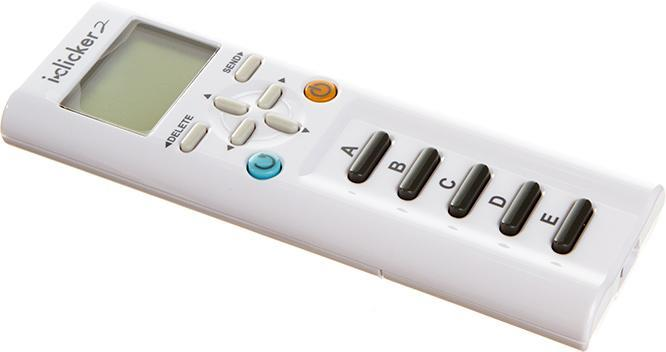
\includegraphics[width=\textwidth]{iclicker.jpg}}
        %\missingfigure{iClicker - An example of an iClicker}
	\caption[iClicker2]{One example of a clicker device called the iClicker2.}\label{fig:iclicker}
\end{figure}

The device depicted in figure \ref{fig:iclicker} is a hardware based CRS, that connects to a receiver in the classroom, that is connected to the teachers computer. The computer can then display the data with a piece of software designed for the system.

A typical hardware based CRS system like the one mentioned above introduces a variety of pros and cons. This includes the investment of buying the system, the receiver and possible licenses for using it could become a large expense. Also there are potential risks, that setting up the system could become a hassle, if the software for example is not maintained for more than one platform or the hardware is difficult to setup. With the emerging of smartphones and fast, reliable internet connections, it could seem like a natural progression to utilize the devices that the users already own, cutting away the expense of buying clicker devices. The users would then use their smartphones or laptops to respond, instead of using a clicker. The concept has been dubbed \emph{Bring Your Own Device} or \emph{BYOD} \cite<Johnson et al., 2013 in>[p.~329]{stowell2015use}. Such systems exists in a variety of different forms, implemented with mixed results. Making the move from the physical to a digital based platform, introduces a whole new range of possibilities and challenges.

There are a variety of examples of online CRS systems. Some are made mainly for children or ground-schoolers\footnote{\url{https://kahoot.it}}, and others are feature rich, made for conferences and classrooms\footnote{\url{http://socrative.com}} \footnote{\url{https://www.polleverywhere.com}} \footnote{\url{https://www.iclicker.com/}}. The most appealing, and seemingly well implemented system is Mentimeter\footnote{\url{https://www.mentimeter.com}}.

Much of the available existing literature about CRS is focused on physical clicker devices and the learning outcomes/improvements of using them. It's less common to find research where the main focus is web based systems, even though smartphones has become widespread and more popular among students \cite[p.~329]{stowell2015use}.

Our own experience shows that it can be problematic when the teacher wants to ask questions which include code. This is hard to do on hardware based devices, and different workarounds where questions are asked on slideshows and answered on clickers are common. We will therefore develop a system that supports showing code and math and test whether or not it's capable of increasing interaction and improving the learning outcome. The research question of this project is:

\begin{quote}
We wish to investigate whether a Classroom Response System that is enhanced for IT educational purposes, is able to enhance classroom interactivity and thereby increase the learning outcome. 
We wish to evaluate the system by gathering empirical data by conducting a pre and post survey on students using our system.
\end{quote}

We wish to gain knowledge on how the market is structured today. By using Porters Five Forces \cite{porter2008five}, we will identify possible culprits that we should be aware about when creating such a system, for it to be competitive.

We will then describe the system that we have developed in two parts. First a general introduction to the system. Secondly a technical description of the specific implementation.
We will then perform a test in two different courses: \emph{Frameworks and Architectures for the Web} and \emph{Advanced Programming}, and discuss our results from the test and show how each CRS performs compared to each other in the two different courses.



% It would seem that the obvious approach would be to leverage the technology that students already own and use. At the IT University of Copenhagen (ITU), laptops are mandatory and free internet access is provided by the university. 

% Each system has a different focus, and how deeply integrated they are varies. Some systems simply wants to ask questions, others wants to grade assignments or provide feedback as well. Though few of them seem to have focus on IT learning specifically, and the ones implementing features that do, lack in other ways.



 \clearpage
\todo{Det her er det samme som "Background" - måske}\section{Existing literature and solutions} % What is already known and done + existing solutions?

%%% Some intro to this maybe...
In this section we will describe different studies and findings from existing literature in order to provide insights of the field of classroom response systems. These insights will help us understand how previous work has been done and how we can evaluate our solution. Furthermore, we will include a description of significant existing solutions in order to compare their features. This comparison will tell us what's missing from existing solutions and which problems we will address.


\subsection{Literature and research} %about CRS}

The following section will include findings, results and mentions of some of the most significant research in the field of response systems in classrooms. Furthermore, this section will mention research based response systems developed at MIT and University of Lugana.

Some of the least resent literature dating back to around 2007, is mainly focused on physical clicker devices, where the students buy actual "remote controls" for polling, in a time where more modern solutions (including the smartphone) has not yet matured. And even today, the physical clicker devices still seem to play a significant role in the \emph{"clicker community"}. \citeA{stowell2015use} explains how the use of clicker systems on physical devices has a greater response rate compared to mobile, but with no significant differences in the final grades of the students. Also, the introduction of students bringing their own devices (the so called \emph{Bring Your Own Device}) introduces new issues such as loss of internet connectivity and the risk of being distracted by the device itself (pp. 331-332).


One of the main reasons to use a CRS is the importance of interactivity in learning \cite{draper2004increasing}. Studies find that CRS engages interactivity, helps students stay active during lectures \cite[p.~116]{moredich2007engaging}, improves learning \cite<e.g.,>{siau2006use, yourstone2008classroom} and increases attention \cite[pp.~86-88]{sun2014influence}. While \citeA{yourstone2008classroom} focuses on actual results in learning outcomes and \citeA{sun2014influence} uses brainwave analysis to determine level of attention while using CRS, most other studies take on a qualitative approach and evaluate teachers and students by asking to their engagement, participation and learning outcomes \cite<e.g.,>{moredich2007engaging}. The latter approach seems to be the most widespread in the literature and focuses more on whether or not students feel an increased engagement and participation rather than their actual performance and examination results. 


\citeA{stowell2007benefits} takes on the qualitative approach where they ask into students emotions towards an introductory psychology class before, during and after lecture. The study compares standard lectures to hand raising, response card and "clicker" lectures\footnote{Standard lectures are thought of as normal lectures where the teacher asks open ended questions to the students. Hand raising is the approach where students are asked to raise their hand if they agree to a statement. Response cards are cards labeled A, B, C, D and are sort of the same as hand raising \cite[p.~254]{stowell2007benefits}.}.
They find that more correct answers to questions are present in response card lectures but explains the much higher correctness with the ability to see what peers are answering \cite[p.~257]{stowell2007benefits}. The same applies for hand raising. Furthermore the study finds that there's a small positive impact on emotions towards the class depending on which kind of lecture is taught (i.e. standard, hand raising, response card and "clicker") \cite{stowell2007benefits}.

One study found that there wasn't a framework for measuring interactivity in classrooms \cite[p.~400]{siau2006use}. They then designed a test framework which consists of a \emph{pretest}, \emph{implementation}, \emph{posttest} and \emph{qualitative data collection}. The pretest is done before starting using a classroom response system. The posttest asks the same questions as the pretest which are then compared to measure difference in interactivity. The posttest, which is done at the end of the course, asks further into the technology and the response system used in the classroom and how the it's perceived \cite{siau2006use}. The implementation is simply the implementation of the response system in the class which are done after the pretest. Finally, the qualitative data collection asks into advantages and disadvantages of using a response system. Their study found a significantly increased interaction reported by the students who participated \cite[p.~400]{siau2006use}. The increase measured on an individual and general level. 


Among the biggest studies of CRS is \emph{Increasing interactivity in lectures using an electronic voting system} by \citeA{draper2004increasing}. This particular study took place over a two year period and found (among other things) that the benefits increases as teachers became aware how to exploit the pedagogy behind the system \cite[p.~93]{draper2004increasing}. The study took place in a time where there was a need for physical hardware (e.g., remote controllers and receivers) in order to facilitate a CRS. This study addresses the need to learn how to proper use a CRS in order to get the benefits from it.

The next parts will focus on some articles which describes and study some different kind of response systems. The studies take on different approaches at teaching computer science and the response systems include atypical features.

All of the before mentioned studies have either not specified which system was used or they used one of the traditional systems available such as the iClicker. Another type of CRS we've found called \emph{Informa} focuses mainly on teaching Java \cite{Hauswirth09}. The system is a software based solution made in Java. The system consists of two different clients; an instructor client and several student clients \cite[p.~1]{Hauswirth09}. Informa is different because it's not a traditional response system, but a task based peer-grading system where the instructor creates a task which the students then are supposed to solve. Students who finish early can grade other students solutions while waiting for everyone to finish \cite{Hauswirth09}. One of \citeA[p.~9]{Hauswirth09}'s findings are that students find the system useful but it's unsure if the system is more useful for the weaker or stronger students. \emph{Informa} is worth mentioning because it is not a typical response system and because it bridges the gap between classroom response systems and teaching a programming language. However, it seems to be limited to teaching Java and can thus not be used to teach other type of courses.

A similar approach can be found in the pen-and-tablet based system that has been used to teach introductory computer science at MIT \cite{koile2007supporting}. The system is called \emph{Classroom Learning Partner} and is a response system where the students answer to question by writing with a pen on a tablet. The hand-written answer is recognized and interpreted by the system, but not without difficulties \cite[pp.~2-3]{koile2007supporting}. A previous study found that their system could improve learning in a CS1 (Computer Science 1) class \cite{koile2006improving}. The study introduced one of two classes to the tablet based system after the first exam (in week 5 of 15) \cite[pp.~6-7]{koile2006improving}. The class not using the system functioned as control group \cite[pp.~6-7]{koile2006improving}. By comparing the score of the students in the different classes their preliminary results showed a difference between the two, where the tablet-PC class performed slightly better \cite{koile2006improving}. They also report that fewer than expected students performed poorly in the tablet-PC class, where \emph{"23.5\% of non-Tablet-PC students were in the bottom 25\% of the class, vs. 6.0\%."} \cite[p.~7]{koile2006improving}. % The significance was p < .05. \clearpage
\section{Competitive Analysis}
To get an overview of the different systems from a competitive standpoint, we introduce an objective analysis based on a list of heuristics that we find relevant based on our initial research within the field of CRS. The heuristics are based upon the common features and functionalities that are seen in the different systems. The list of CRS are based on our own field research. A substantial amount of time has been spent on finding these systems, and the ones mentioned here covers a great deal of the CRS'es that are available today.

\subsection{Heuristics}

The following is a list of the chosen heuristics.

\begin{itemize}
    \item Web/Software/Hardware based
    \item Multiple question types
    \item Multiline question and answers
    \item Math notation
    \item Source code notation
    \item Supports image upload as questions
    \item Timed questions/auto closing questions
    \item Payment model
\end{itemize}

The first heuristic determines if the system is web, software or hardware based. Some systems are only accessible online, while others are purely hardware based, and users needs to purchase specific hardware for it to work. A few systems are also purely software based, and is created for use on computers, and does not have any specific hardware.

Many CRS offers multiple types of questions. An example is one of the more common ones, the quiz, also known as the multiple choice question where users can select an answer, and one (or more) of those answers are correct.

Some CRS offers the possibility to ask questions with multiple lines of text. This enables teachers to ask questions spanning several lines, useful in certain scenarios. The same principle is applicable to answers.

Math notation is used for asking questions and choosing answers with mathematical expressions. This means that the system supports the ability to show formulas formatted like this: $$x = {-b \pm \sqrt{b^2-4ac} \over 2a}$$

Source code support is defined as a system that supports (at a minimum) the ability of multiline questions and answers, and uses a monospaced font for it. 

Image upload is the possibility to upload an image as a question. This enables the users to use any format for a question, since they can simply upload an image that looks exactly the way they want it to.

Timed questions enables the users to auto close questions after a certain amount of time. In some cases the remaining time available to answer the question is visible to the responders.

The payment model differ from system to system. We will not go into details about pricing, but 


All the following CRS will be analysed with these heuristics taken into consideration.

\subsection*{Kahoot}
Kahoot is a web based CRS, that focuses on teaching children. Kahoot themselves states that  \emph{"it gives students a voice in the classroom, and allows educators to engage and focus their students through play and creativity"} \footnote{Retrieved on 2016-3-25 \url{https://getkahoot.com/support/faq/\#is-kahoot-a-social-media-tool}}. Kahoot is purely web based and supports multiple question types such as quizzes, discussions and surveys. It has image upload support to make questions more engaging, but it does not support multiline questions and answer, nor does it have support for math notation and source code highlighting. It does have timed questions though. Even though Kahoot works well, it is only created with simple questions in mind, that would fit in one line, also the colorful design is appealing for an audience of younger age. Kahoot is free to use and has no payment options.

\subsection*{Socrative}
Socrative is a web based platform that supports multiple question types. It has support for multiline question and answers, but not for monospaced fonts, thus math notation and source code notation is not directly supported. There is support for imageupload, so it's possible to see an image as a question. The system is a so called \emph{K-12} solution, which means it is build for elemanty to high schoolers. Socrative is free to use, but does reserve the right to introduce payed extra features.

\subsection*{Poll Everywhere}
Poll Everywhere is a response system with several different possibilities for voting. You can \emph{"(...) respond via the poll's web page on PollEverywhere.com, or via an embeddable voting widget, or on a mobile web browser using PollEv.com, or even through Twitter"} beside sending a text to a specified number\footnote{Retrieved on 2016-3-25 \url{https://www.polleverywhere.com/faq\#how-to-vote}}. Poll Everywhere will primary be web based since questions are created on their web page. The system support different kind of questions such as multiple choice, open ended questions, clickable images and it has a Q\&A/brainstorming feature. Furthermore, Poll Everywhere has the possibility of displaying short single lines of Latex and thus displaying math. A blog post on their site from 2012 contains a video which shows how to insert Latex at the very end of the video\footnote{Retrieved on 2016-3-25 \url{http://www.polleverywhere.com/blog/its-what-you-wanted-image-support-math-equati/}}. It has been impossible to find the information anywhere else.

Poll Everywhere doesn't support multiple lines in their questions and answers, and nor does it support source code in the questions/answers. It does support images as answer but not as a question. It's not possible to time questions on Poll Everywhere and it's only possible to have one active question at any time. 

\subsection*{iClicker}
iClicker started out as a purely hardware based CRS, but has recently updated their solution with a web based platform for answering as well (including apps for iOS and Android devices). This means that teachers still need a piece of software, but students can use a web based platform for responding. It supports multiple question types. The iClicker software is capable of sending a screendump from the teachers computer to the web application (or app), thus enabling the teacher to use any software of their choosing for asking questions. In principle this enables multiline questions and math/source code notation. 

\subsection*{Mentimeter}
Mentimeter is a purely web based platform and also one of the more feature rich. It supports seven different question types, but does not have any multiline support. It does however offer a description field for each question, but it is limited to 100 characters making more complex question asking hard to do. Even though Mentimeter is very feature rich, it does not have support for math notation, nor does it have source code notation.  Image upload is not supported, but timed questions are in 2 varieties. Mentimeters payment model is subscription based, with several types of subscriptions. 

\subsection*{Tophat}
Tophat is similar to Mentimeter and Poll Everywhere in form and function. It's a web based solution capable of taking attendance and asking questions. Tophat features 6 different question types, a discussion function and a tournament mode which let students compete against each other. Tophat supports displaying math and code by including tags like [math]\emph{some equation}[/math] and [code]void main()[/code]. Code is simply displayed in a grey box with black text and is not highlighting any syntax. This also implies that it's possible to ask multiline questions. However, it's not possible to create multiline answers. It's possible to set a timer on questions in order to change the status from active (labeled as "Homework") or review to review and closed. Tophat features a few more statuses but these cannot be used when scheduling a question. In order to use Tophat, every student must pay a fee corresponding to how long they intend to use the system.

\subsection*{Learning Catalytics}
Learning Catalytics is a solution made by Pearson. The system seems feature rich from instruction videos and guides, but it's not possible to test for ourselves since it's behind a pay wall. Learning Catalytics seems to be software and web based from videos found at their website\footnote{Retrieved on 2016-03-28 \url{https://learningcatalytics.com/pages/training}}. The videos also reveal an advanced grading system based on how many tries it took to answer the correct answer. Learning Catalytics features options for the instructor to make a seat map which is supposedly used to tell students who to team up with when solving group exercises. An "I don't understand this"-button can be pressed to tell the instructor that you don't understand the material taught or the question asked. In order to use Learning Catalytics, students or their institution must pay for a subscription while instructors can use it for free.

\subsection*{Informa}
Informa is a system and tool for teaching Java. It's build and tested at University of Lugano. Informa is a traditional response system while it supports teaching Java with different approaches and techniques. For example: It's possible to ask students to highlight specific parts of some provided code or determine types of already highlighted code \cite[p.~2]{Hauswirth09}. Furthermore the system supports a method for asking students to draw diagrams and flowcharts \cite[p.~3]{Hauswirth09}. 
The system consists of two different clients, an instructor client and several student clients. 

\subsection*{Renaissance}
Renaissance is a hardware and software based system where users respond using the \emph{Renaissance Responder}. It is a simple multiple choice system, so multiple question types are not directly supported. Answers are limited to A,B,C,D and E and True or False via the responder hardware, multiline questions and answers are therefore not supported. Math notation is not possible but the system does have a build in calculator. Source code notation and image upload is not supported. It is unclear if timed questions are supported, as the documentation for the system is sparse, but based on the other features of the systems it is not likely. The payment model for the system is based on hardware purchases.

\subsection*{Classroom Learning Partner}
The Classroom Learning Partner (CLP) is a software based system where \emph{"the goal of the [...] project is to increase instructor-student interaction and student learning in large classes by developing software to support the use of in-class exercises"} \footnote{Retrieved on 2016-03-29 \url{http://publications.csail.mit.edu/abstracts/abstracts07/kkoile/kkoile.html}}. The system is different from the other mentioned ones, in terms of input type, where CLP relies heavily on written input, the so called \emph{Digital Ink} input, or simply hand written input \cite{koile2007supporting}. The system supports multiple question types and also multiline questions. It is unclear wether the system supports mathematical notation, but it does support source code, since the text font is a monospaced font. It's possible to upload images, and even draw the questions. Timed questions are not available.



\subsection*{Shakespeak}
Shakespeak is the type of response system that uses traditional software in order to work. Unfortunately it will only run on Windows. Shakespeak integrates directly into Microsoft PowerPoint and adds an extra menu. From here it's possible to ask questions to an audience. In order to vote or answer a question created with Shakespeak, the responder can text, answer online or send a tweet with Twitter \footnote{Retrieved on 2016-04-01 \url{https://www.shakespeak.com/how-to-use-shakespeak-during-all-your-presentations/}}. It supports two kinds of questions: multiple choice and open questions. Since the response system lives directly in PowerPoint, it will potentially be possible to ask questions with math, source code and images. It's possible to use Shakespeak for free with a limitation on the amount of users who are allowed to answer questions.




%    \item Web/Software/Hardware based
%    \item Multiple question types
%    \item Multiline question and answers
%    \item Math notation
%    \item Source code notation
%    \item Supports image upload as questions
%    \item Timed questions/auto closing questions
%    \item Payment model


\begin{landscape}
    \begin{center}
        \begin{table}[H]
            \begin{tabularx}{\paperwidth}{ |X|X|X|X|X|X|X|X|X| } 
             \hline
                 & Web \newline Software \newline Hardware based & Multiple question types & Multiline support & Math notation & Source code notation & Supports image upload as questions & Timed questions/auto closing questions & Payment model \\ \hline
                 
              Kahoot                & Web   & No    & No    & No    & No    & Yes   & Yes   & Free \\ \hline
              Socrative             & Web   & Yes   & Yes   & No    & No    & Yes   & No    & Free \\ \hline
              Poll Everywhere       & Web   & Yes   & No    & Yes   & No    & Yes   & Yes   & Subscription \\ \hline
              iClicker              & All   & Yes   & No    & No    & No    & Yes   & No    & Mixed based on solution \\ \hline
              Mentimeter            & Web   & Yes, 7 & No   & No    & No    & No    & Yes   & Subscription \\ \hline
              Tophat                & Web   & Yes, 6 & Questions only & Yes & Yes   & No    & Yes & Subscription \\ \hline
              Learning Catalytics   & Web, software   & Yes    & Yes  & N/A   & N/A   & Yes   & N/A   & Subscription \\ \hline
              Informa        & Software & Yes & Yes  & No & Yes   & No    & No    & Research project, free \\ \hline
              Renaissance           & Software \newline Hardware & Yes & No & No & No & N/A & No & Hardware purchase \\ \hline
              Classroom Learning Partner & Software \newline Hardware & Yes & Yes & No & Yes & Yes & No & Research project, not sold \\
             \hline
             Shakespeak & Software \newline Web & Yes, 2 & Yes & (Yes) & (Yes) & (Yes) & No & Subscription \\
             \hline
            \end{tabularx}
            \caption{Overview of different systems}\label{tab:overview}
        \end{table}
    \end{center}
\end{landscape}





 \clearpage
\section{System description}\todo{Make it fit, baby}
The system can be described as a Classroom Response System (CRS) in the sense that it's a system made for polling and gathering responses in a classroom.

The system includes features that support asking and answering technical questions\footnote{Here we've defined technical questions as questions that can display formatted code and mathematical expressions.}. Here we'll give an explanation of how to use the system and how the different parts 


\subsection{Rooms}
A room is a collection of groups, and any user can create a room. The use of the term \emph{room} could be resembled with a classroom. In order to subscribe to a room, you may search for it using the search field in the menu bar. A blank search will show you every room available, and you may subscribe directly from the search results. It is also possible to simply obtain the rooms URL, and subscribe to it from there.


\subsection{Groups and Questions}
Within a room you'll find groups which is a collection of questions (hence a group). These groups are included in order to structure questions. There could be multiple reasons to why you would group questions together. One could be that you would want to make a group of questions public at once. Another reason could be that you would like to keep questions from each lecture separated in groups.

In order to control which groups and questions are open for answers, we made a feature that would let the owner control the access. This is done by pressing open/close on groups and question. Subscribers of a room will be able to see closed groups but not the belonging questions. If a group is open, subscribers will be able to see the question but not answering them unless the questions are open as well.

%% Main features
The main feature of the system consists of creating and answering questions. When you create a new question, you are presented with an option to create one or more answers.
These features are almost identical in every similar response system, and is part of the definition of the basic functionalities in a CRS \todo{SE BILAG FOR EN LISTE OVER CRS MÅSKE?}

When creating and editing questions, we have made it possible to include code and mathematical expression in questions and answers. Code will be nicely formatted with the Prettify library \cite{google/code-prettify_2016} and mathematical expressions will be shown with the MathJax \cite{mathjax_2016}. This eliminates the need for using different systems to ask a question when you want to include code or math. To show code, it is necessary to add \texttt{<pre>} tags around the code to add line numbers and syntax highlighting. The Prettify-library will automatically determine the language and highlight it accordingly. When writing mathematical expressions into a question or answer, the creator will have to use the same syntax as in \LaTeX. That would mean that an expressions like \verb|$a \ne 0$| would be translated into $a \ne 0$ and \verb|$$x = {-b \pm \sqrt{b^2-4ac} \over 2a}$$| would be $$x = {-b \pm \sqrt{b^2-4ac} \over 2a}$$
This is meant to be convenient for people already knowing and using \LaTeX.

In theory, the system supports adding unlimited answers to a question. The only criteria is that an answer can't be left empty by the creator. The creator of a question have the ability to mark one or more answers as correct. This will make subscribers able to track their performance and see whether they answered correctly or not. It's also possible not to mark an answer as correct if the system is simply used for polling, and there are no correct answer.

When responses are received to a question, the owner can track what is being answered in real time. When enough responses are received, the owner can then close the question and the subscribers will be able to see the responses as well. Responses are shown with a chart which describes how many have chosen each answer. 


%\subsection{}
%When deciding what features to include in the system, we've also decided which features not to %include. Some 
 \clearpage


%--------------------REFERENCES--------------------%
\bibliographystyle{apacite}
\bibliography{references.bib}
%--------------------REFERENCES--------------------%

\end{document}
